\documentclass[aspectratio=169]{beamer}
\usepackage{tikz}
\usepackage{graphicx}
\usepackage{listings}
\usepackage{xcolor}
\usepackage{hyperref}
\usepackage[spanish,es-noquoting]{babel}
\usepackage[round]{natbib}

\lstset{
  basicstyle=\ttfamily\small,
  keywordstyle=\color{blue},
  stringstyle=\color{red},
  commentstyle=\color{gray},
  showstringspaces=false
}
% Minimal look
\usetheme{Warsaw}
%\setbeamertemplate{headline}
\setbeamertemplate{footline}{
  \leavevmode%
  \hbox{%
    % Left: Section name
    \begin{beamercolorbox}[wd=.33\paperwidth,ht=2.25ex,dp=1ex,left]{author in head/foot}%
      \hspace*{2ex}\insertsection
    \end{beamercolorbox}%
    % Center: Presentation title
    \begin{beamercolorbox}[wd=.34\paperwidth,ht=2.25ex,dp=1ex,center]{title in head/foot}%
      \insertshorttitle
    \end{beamercolorbox}%
    % Right: Slide numbers
    \begin{beamercolorbox}[wd=.33\paperwidth,ht=2.25ex,dp=1ex,right]{date in head/foot}%
      \insertframenumber{} / \inserttotalframenumber\hspace*{2ex}
    \end{beamercolorbox}%
  }%
  \vskip0pt%
}

\usecolortheme{default}
\usefonttheme{serif}
\graphicspath{{../}{./}}
\setbeamertemplate{caption}[numbered]

% Title info
\title[ Masterclass]{ Masterclass: Integración de Fundamentos y Frameworks Avanzados}
\subtitle{ Casos prácticos y aplicación intensiva (Sesión 3 - 2 Horas)}
\author{Ricardo Reyes-Jimenez}
\institute{Universidad de La Sabana}
\date{\today}

% Background image for title slide
\usebackgroundtemplate{
  \tikz\node[opacity=0.3]{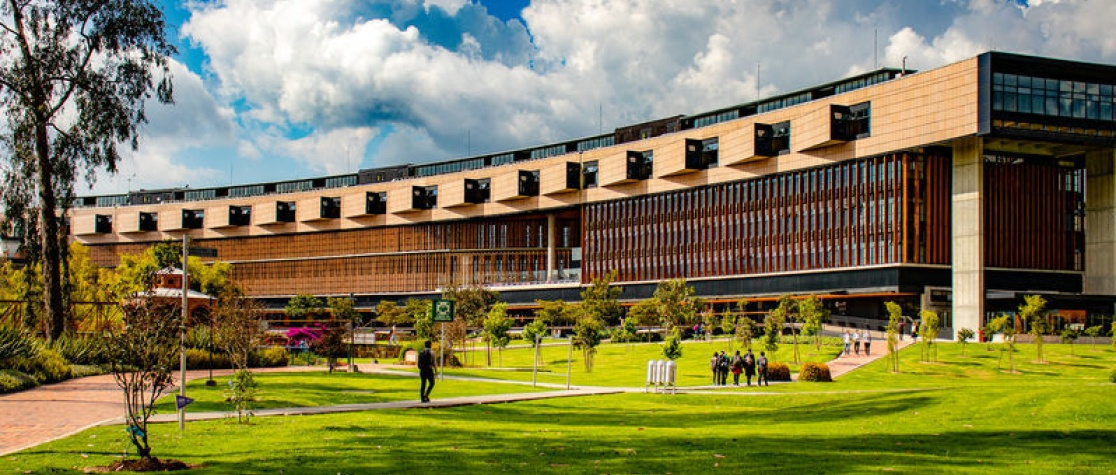
\includegraphics[width=\paperwidth,height=\paperheight]{Images/UniSabana.jpg}};
}

\begin{document}

% Title slide
\begin{frame}
  \titlepage
\end{frame}

% Reset background for normal slides
\usebackgroundtemplate{}



\begin{frame}[fragile]{Objetivos de la Masterclass (2 Horas)}


\begin{itemize}
  \item \textbf{Visión Integradora (15 min):} Combinar los 5 componentes base con los frameworks avanzados.
  \item \textbf{Caso Práctico 1 (30 min):} Elaboración de Conceptos Complejos (CARE + Few-Shot).
  \item \textbf{Caso Práctico 2 (30 min):} Auditoría y Blindaje de Contratos (ADP + Red Teaming).
  \item \textbf{Caso Práctico 3 (30 min):} Estrategia de Litigio paso a paso (CoT + Break the Task Down).
  \item \textbf{Taller Integrador (15 min):} Resolución de dudas y cierre.
\end{itemize}
\end{frame}



\begin{frame}[fragile]{Repaso: La Fusión de Técnicas}


Para resolver problemas jurídicos complejos, no basta una sola técnica. Debemos combinar:

1. \textbf{La Estructura Base:} Rol + Contexto + Instrucción + Restricciones + Formato.
2. \textbf{El Razonamiento (CoT):} Pedirle a la IA que piense paso a paso.
3. \textbf{El Framework:} Usar CARE para conceptos, ADP para auditar o TAM para comunicar.
4. \textbf{El Estilo (Few-Shot):} Darle ejemplos de cómo escribimos.

\textbf{Fórmula del Éxito:} `Estructura Base + Framework (CARE/ADP) + CoT + Few-Shot = Prompt Maestro`

\end{frame}



\begin{frame}[fragile]{Caso 1: Conceptos Tributarios Complejos}


\textbf{El Reto:} Redactar un memorando sobre implicaciones fiscales de una fusión, manteniendo el tono de la firma.

\textbf{Estrategia:} Combinar el Framework \textbf{CARE} con \textbf{Few-Shot Prompting}.

\begin{itemize}
  \item \textbf{C - Contexto:} Datos de las empresas que se fusionan.
  \item \textbf{A - Acción:} Analizar la viabilidad y riesgos.
  \item \textbf{R - Resultado:} Memorando formal.
  \item \textbf{E - Evaluación:} Restricciones legales (Estatuto Tributario).
  \item \textbf{+ Few-Shot:} Incluir ejemplos de memorandos previos.
\end{itemize}
\end{frame}



\begin{frame}[fragile]{Caso 1: El Prompt Maestro (CARE + Few-Shot)}


\begin{lstlisting}[basicstyle=\ttfamily\scriptsize]
[ROL]: Eres un Socio de Impuestos en Colombia con 20 años de experiencia.

[CONVENIO CARE]
1. CONTEXTO: Empresa A (colombiana) absorbe a Empresa B (española). Hay activos intangibles involucrados.
2. ACCION: Elabora un concepto sobre las implicaciones en el impuesto sobre la renta por la transferencia de intangibles.
3. RESULTADO: Memorando ejecutivo con titulos y viñetas.
4. EVALUACION: Limitate al Estatuto Tributario colombiano y convenios de doble imposicion. No analices temas laborales.

[EJEMPLOS DE ESTILO (FEW-SHOT)]
Ejemplo de nuestro tono: ``De conformidad con el articulo X del ET, es imperativo estructurar...'' (Evita lenguaje coloquial).
\end{lstlisting}


\end{frame}



\begin{frame}[fragile]{Caso 2: Auditoría y Blindaje de Contratos}


\textbf{El Reto:} Revisar un contrato de arrendamiento comercial leonino y prepararse para negociar.

\textbf{Estrategia:} Combinar el Framework \textbf{ADP} con \textbf{Red Teaming}.

\begin{itemize}
  \item Primero, usamos ADP para que la IA actúe como nuestro abogado auditor.
  \item Luego, usamos Red Teaming para que la IA actúe como la contraparte y ataque nuestros propios argumentos.
\end{itemize}
\end{frame}



\begin{frame}[fragile]{Caso 2: El Prompt Maestro (ADP + Red Teaming)}


\textbf{Paso 1: Auditoría (ADP)}
\textit{[ACTOR]: Eres el abogado del Arrendatario.}
\textit{[DOCUMENTO]: [Insertar texto del contrato]}
\textit{[PROPÓSITO]: Identifica cláusulas penales abusivas y renuncia a requerimientos. Sugiere redacción alternativa para mitigarlo.}

\textbf{Paso 2: Blindaje (Red Teaming)}
\textit{[INSTRUCCIÓN]: Ahora, cambia de rol. Actúa como el abogado del Arrendador. Revisa las redacciones alternativas que acabas de sugerir y encuéntrales 3 debilidades jurídicas. ¿Cómo te negarías a aceptarlas en una negociación?}


\end{frame}



\begin{frame}[fragile]{Caso 3: Estrategia de Litigio Paso a Paso}


\textbf{El Reto:} Evaluar si vale la pena iniciar una demanda por despido injustificado con pruebas contradictorias.

\textbf{Estrategia:} Combinar \textbf{Break the Task Down} con \textbf{Chain-of-Thought (CoT)}.

\begin{itemize}
  \item Dividir el análisis en fases lógicas (hechos, pruebas, norma, conclusión).
  \item Obligar a la IA a mostrar su razonamiento paso a paso antes de decidir.
\end{itemize}
\end{frame}



\begin{frame}[fragile]{Caso 3: El Prompt Maestro (CoT)}


\begin{lstlisting}[basicstyle=\ttfamily\scriptsize]
[ROL]: Eres un Juez Laboral del Circuito.
[CONTEXTO]: [Insertar hechos del despido y pruebas testimoniales cruzadas]

[INSTRUCCION]:
Analiza la probabilidad de exito de una demanda laboral.
NO ME DES LA CONCLUSION TODAVIA. Sigue estrictamente este orden de razonamiento paso a paso (Chain-of-Thought):
1. Califica la validez de cada prueba individualmente.
2. Identifica si hay justa causa segun el Codigo Sustantivo del Trabajo.
3. Analiza las contradicciones en los testimonios.
4. Solo despues de los 3 pasos anteriores, redacta tu veredicto de probabilidad de exito (Alto, Medio, Bajo) justificando el por que.
\end{lstlisting}

\end{frame}



\begin{frame}[fragile]{Taller Práctico Integrador (45 Minutos)}


\textbf{Dinámica:}
1. Divídanse en grupos de 3 personas.
2. Elijan un caso real y complejo (ej. estructuración corporativa, defensa penal, o cobro pre-jurídico).
3. Construyan un \textbf{Prompt Maestro} que fusione la estructura de 5 componentes con al menos dos frameworks vistos (ej. CARE + CoT).
4. Ejecuten el prompt en su IA de preferencia.
5. Apliquen \textbf{Red Teaming} a la respuesta.

\textbf{Entregable:} Compartir con la clase el prompt inicial, el resultado y cómo lo mejoraron.

\end{frame}



\begin{frame}[fragile]{Criterios para Evaluar sus Prompts Maestros}


\begin{itemize}
  \item \textbf{Estructura:} ¿Tiene los 5 componentes claramente definidos?
  \item \textbf{Razonamiento:} ¿Se le dio espacio a la IA para ``pensar'' antes de concluir (CoT)?
  \item \textbf{Estilo:} ¿Se incluyeron directrices de tono o ejemplos (Few-Shot)?
  \item \textbf{Red Teaming:} ¿Sometimos el entregable a una evaluación crítica simulando a la contraparte?
\end{itemize}
\end{frame}



\begin{frame}[fragile]{Conclusión y Cierre del Módulo 2}


\textbf{Resumen:}
1. Pasamos del ``buscador de Google'' a dar instrucciones delegadas precisas.
2. Entendimos que la IA es probabilística y necesita restricciones para no alucinar.
3. Aprendimos frameworks (CARE, ADP, TAM) para estandarizar el trabajo.
4. Dominamos la ingeniería de razonamiento (CoT, Red Teaming) para tareas complejas.

\textbf{Próximos Pasos:} Apliquen hoy mismo un prompt maestro en su trabajo. Guarde sus mejores prompts en un documento compartido con su equipo.

\textbf{¡Gracias por su dedicación en este módulo!}
\end{frame}




\begin{frame}[allowframebreaks]{Referencias}
  \bibliographystyle{apalike}
  \bibliography{references}
\end{frame}


\end{document}